\section{Overlaying Arrangements\label{arr_sec:overlay}}
%================================

Assume that we are given two geographic maps represented as
arrangements with some data objects attached to their faces,
representing some geographic information --- for example, a map of
the annual precipitation in some country and a map of the vegetation
in the same country. It is interesting to overlay the two maps to
locate, for example, the regions where there is a pine forest and
the annual precipitation is between 1000\,mm and 1500\,mm. 

Computing the overlay of two planar arrangement is also useful for
supporting Boolean set operations on polygons (or generalized polygons,
see, e.g.,~\cite{cgal:behhms-cbcab-02}).

The function \ccc{overlay (arr_a, arr_b, ovl_arr, ovl_traits)} accepts
two input arrangement instances \ccc{arr_a} and \ccc{arr_b}, and constructs
their overlay instance \ccc{ovl_arr}. All three arrangements must use the
same geometric primitives. More precisely, let \ccc{arr_a} be of 
type \ccc{Arrangement_2<Traits_A,Dcel_A>}, \ccc{arr_b} be of type
\ccc{Arrangement_2<Traits_B,Dcel_B>} and the resulting \ccc{ovl_arr} be of type 
\ccc{Arrangement_2<Traits_R,Dcel_R>}. All types nested in geometry
traits \ccc{Traits_A}, e.g., \ccc{Point_2} and
\ccc{X_monotone_curve_2}, must be convertible to the corresponding 
types nested in geometry traits \ccc{Traits_R}. The same holds for all
types nested in geometry traits \ccc{Traits_B}.
The \ccc{ovl_traits} parameter is
an instance of an {\em overlay traits-class}, which enables the creation of
\ccc{Dcel_R} records in the overlaid arrangement from the \dcel\ features
of \ccc{arr_a} and \ccc{arr_b} that they correspond to.

In principle, we distinguish between three levels of overlay:
\begin{description}
\item[Simple overlay:]
An overlay of two arrangements that store no additional data
with their \dcel\ records. That is, they are defined using the default 
\dcel\ class \ccc{Arr_default_dcel}. Typically, the overlaid
arrangement in this case stores no extra data with its \dcel\ records as
well (or if it does, the additional data fields cannot be computed by
the overlay operation), so by overlaying the two arrangement we just
compute the arrangement of all curves that induce \ccc{arr_a} and \ccc{arr_b}.
Note that the same result can be obtained using the standard insertion
operations, but users may choose to use overlay computation in order to
achieve better running times.

The \ccc{Arr_default_overlay_traits} class should be used as an overlay
traits-class for such simple overlay operations.
%
\item[Face overlay:]
An overlay of two arrangements that store additional data
fields with their faces (e.g., the geographic-map example
given in the beginning of this section). The resulting overlaid arrangement
typically also stores extraneous data fields with its faces, where the
data field that is attached to an overlaid face can be computed from the
data fields of the two faces (in \ccc{arr_a} and \ccc{arr_b}) that induce
the overlaid face.

The \ccc{Arr_face_overlay_traits} class should be used as an overlay
traits-class for face-overlay operations. It operates on arrangement, whose
\dcel\ representation is based on the \ccc{Arr_face_extended_dcel}
class-template (see Section~\ref{arr_ssec:ex_dcel_face}). The face-overlay
traits-class is parameterized by a functor that is capable of combining two
face-data fields of types \ccc{Dcel_A::Face_data} and
\ccc{Dcel_B::Face_data}, and computing the output \ccc{Dcel_R::Face_data}
object. The overlay traits-class uses this functor to properly construct
the overlaid faces.
%
\item[Full overlay:]
An overlay of two arrangements that store additional data
fields with all their \dcel\ records. That is, their \dcel\ classes
are instantiations of the \ccc{Arr_extended_dcel} class-template (see
Section~\ref{arr_ssec:ex_dcel_all}), where the resulting arrangement
also extends it \dcel\ records with data fields computed on the basis
of the overlapping \dcel\ features of the two input arrangements.
\end{description}

In the following subsections we give some examples for the simple and the
face-overlay operations and demonstrate how to use the auxiliary overlay
traits-classes. For the full overlay operations users need to implement
their specialized overlay traits-class, which models the \ccc{OverlayTraits}
concept. The details of this concept are given in the Reference Manual.

\subsection{Example for a Simple Overlay\label{arr_ssec:simp_ovl}}
%----------------------------------------

\begin{figure}[t]
\begin{ccTexOnly}
  \begin{center}
  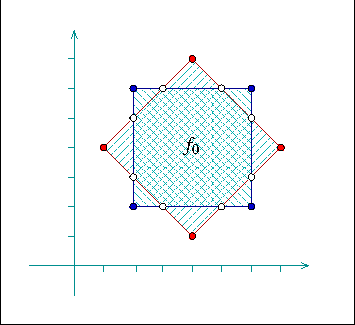
\includegraphics{Arrangement_on_surface_2/fig/ex_22}
  \end{center}
\end{ccTexOnly}
\begin{ccHtmlOnly}
  <p><center>
  <img src="./fig/ex_22.gif" border=0 alt="Example 22">
  </center>
\end{ccHtmlOnly}
\caption{Overlaying two simple arrangements of line segments, as done
in \ccc{overlay.cpp} and \ccc{ex_face_extension_overlay.cpp}.
In \ccc{face_extension_overlay.cpp} the two bounded faces are
considered as {\em marked}, and the octagonal face which is the intersection
of the two marked faces is denoted by $f_0$.\label{arr_fig:ex_22}}
\end{figure}

The next program constructs two simple arrangements, as depicted in
Figure~\ref{arr_fig:ex_22} and computes their overlay:

\ccIncludeExampleCode{Arrangement_on_surface_2/overlay.cpp}

\subsection{Examples for a Face Overlay\label{arr_ssec:face_ovl}}
%--------------------------------------

The following example shows how to compute the intersection of two polygons
using the \ccc{overlay()} function. It uses a face-extended \dcel\ class
to define our arrangement class. The \dcel\ extends each face with a Boolean 
flag. A polygon is represented as a {\sl marked} arrangement face, (whose
flag is set). The example uses a face-overlay traits class, instantiated with 
a functor that simply performs a logical {\em and} operations on Boolean flags.
As a result, a face in the overlaid arrangement is marked only when it
corresponds to an overlapping region of two marked cells in the input
arrangements. Namely, it is part of the intersection of the two polygons.

The example computes the intersection between a square and a rhombus, (which is
actually also a square). The resulting polygon is an octagon, denoted
by $f_0$ in Figure~\ref{arr_fig:ex_22}:

\ccIncludeExampleCode{Arrangement_on_surface_2/face_extension_overlay.cpp}

The next example demonstrates the face overlay of two arrangements that
have unbounded faces as well. The first arrangement is formed by the two lines
$y = x$ and $y = -x$, that subdivide the plane into four unbounded faces,
denoted $A$, $B$, $C$ and $D$. The second arrangement comprises four line
segments that form a square-shaped face. When we overlay the two arrangements,
each of the four faces $A$, $B$, $C$ and $D$ is split into an unbounded
face (indexed 1) and a bounded face (indexed 2):

\ccIncludeExampleCode{Arrangement_on_surface_2/overlay_unbounded.cpp}
